\subsection{Comparison to chemiluminescence measurements}
\label{sec:cld}

After having assured the functionality of the converter in the lab
environment, I wanted to use it with ambient air. I wanted to try out
the alternating measurement mode described in the previous section and
compare the results to another nitrogen monoxide measurement
instrument, a chemiluminescence monitor (or display, short: cld). This
made it possible to work in a more realistic setting while
simultaneously being able to verify the converter results.

\subsubsection{Setup}
\label{sec:cld-setup}

The cavity and the chemiluminescence monitor (Eco Physics CLD 770 AL
ppt Chemiluminescence \ch{NO} Analyzer) were both setup at the rooftop
laboratory at the Institute for Environmental Physics. I used a
tripod on the roof together with two teflon tubes to make sure to
sample at the same spot with both instruments.

I set up the cavity as described in Section~\ref{sec:inclusion}. For
each spectrum I sampled 3000 spectra at an exposure time of
\SI{10}{\milli\second}. Furthermore, I used a purge time of
\SI{30}{\second} after ozone switches. This time was set too short to
account for the slowly falling tail, as Section~\ref{sec:switch}
indicates.

In order to account for slight differences in the path length and
flows in the two instruments, I decided to compute \SI{30}{\minute}
averages for the comparison. These measurements were taken during the
day of January 22 and January 25, 2016.

\subsubsection{Results}
\label{sec:cld-results}

The time series of the two measurements can be found in
Figure~\ref{fig:corr-ts}. As can be seen, the qualitative form of the
DOAS results is in good accordance with the chemiluminescence results.
However, there seems to be an offset and the DOAS concentration is
systematically lower than the chemiluminescence concentration. This
relation is also plainly visible in the correlation plot in
Figure~\ref{fig:cld-corr}. The measurements are very well correlated
and can be easily fitted by a linear regression, but the line has an
offset and a slope, which is differing from unity:

\begin{align*}
  y = \SI{1.38}{{ppb}\tothe{-1}} \cdot x + 3.8.
\end{align*}

There were two avenues I followed in an attempt to understand these
findings. Both of them follow arguments already layed out in
Section~\ref{sec:switch}. The first consists in the observation that
the \ch{NO} calibration gas container was used to calibrate the
chemiluminescence display. If some of the \ch{NO} had been converted
to \ch{NO2}, there would be an error in the chemiluminescence
calibration, which would lead to an overestimation of the \ch{NO}
concentration by the cld. Using the \ch{NO2} offset found in the
previous section, it is possible compute that there is about
\SI{420}{ppb} \ch{NO2} in the cylinder, if all of it stemmed from
\ch{NO} this would introduce an error of about \SI{5}{\percent} (the
calibration concentration given was $c = \SI{8.177}{ppm}$). This is
not enough to explain the discrepancy. Together with the fact that I
still cannot explain, how the transition from \ch{NO} to \ch{NO2}
could occur, I discarded this approach.

The second avenue I took was to look at the purge time.
Section~\ref{sec:switch} suggests that \SI{30}{\second} purge time is
not enough after the ozone switch has been turned off. Thus one would
expect the measured \ch{NO2} intensities to be overestimated. One
observation pointing towards the influence of this effect is, that I
measured negative \ch{NO} concentrations (to a minimum of
\SI{-1.54}{ppb}), which is of course absurd. In the previous section I
suggested that the surplus \ch{NO2} signal does not depend too strongly
on the \ch{NO} concentration. If this assumption is correct, one will
expect to be able to mitigate the effects by lowering the \ch{NO2}
signal by $\bar c_s = \SI{1.55}{ppb}$ (c.\,f.\
Equation~\eqref{eq:offset} on page~\pageref{eq:offset}), which
corresponds surprisingly well to the negative offset of the measured
data. This \emph{tail corrected} data set was then again correlated
with the chemiluminescence data. The result can also be found in
Figure~\ref{fig:cld-corr}. The linear regression follows the formula
\begin{align*}
  y = \SI{1.38}{ppb\tothe{-1}} \cdot x + 1.67.
\end{align*}
So the tail correction has only an effect on the intercept of the
regression. This is expected as the constant lowering of the \ch{NO2}
signal increases the computed \ch{NO} signal by the same amount and
thus all data points are shifted to the right. Hence the slope of the
regression is still off. Clearly, the approach utilized here was too
simplistic to account for all effects. Further investigations are
necessary to understand the required corrections. Possibly, the
\ch{NO2} correction can be computed utilizing the previous \ch{NO_x}
data point, thus indirectly taking \ch{NO} influences on the offset
into account. This varying \ch{NO2} correction could then also
influence the slope of the regression. In order to investigate this
further, I suggest to perform additional decay measurements as
proposed in the previous section.

\begin{figure}[htbp]
  \centering
  % GNUPLOT: LaTeX picture with Postscript
\begingroup
  \makeatletter
  \providecommand\color[2][]{%
    \GenericError{(gnuplot) \space\space\space\@spaces}{%
      Package color not loaded in conjunction with
      terminal option `colourtext'%
    }{See the gnuplot documentation for explanation.%
    }{Either use 'blacktext' in gnuplot or load the package
      color.sty in LaTeX.}%
    \renewcommand\color[2][]{}%
  }%
  \providecommand\includegraphics[2][]{%
    \GenericError{(gnuplot) \space\space\space\@spaces}{%
      Package graphicx or graphics not loaded%
    }{See the gnuplot documentation for explanation.%
    }{The gnuplot epslatex terminal needs graphicx.sty or graphics.sty.}%
    \renewcommand\includegraphics[2][]{}%
  }%
  \providecommand\rotatebox[2]{#2}%
  \@ifundefined{ifGPcolor}{%
    \newif\ifGPcolor
    \GPcolorfalse
  }{}%
  \@ifundefined{ifGPblacktext}{%
    \newif\ifGPblacktext
    \GPblacktexttrue
  }{}%
  % define a \g@addto@macro without @ in the name:
  \let\gplgaddtomacro\g@addto@macro
  % define empty templates for all commands taking text:
  \gdef\gplbacktext{}%
  \gdef\gplfronttext{}%
  \makeatother
  \ifGPblacktext
    % no textcolor at all
    \def\colorrgb#1{}%
    \def\colorgray#1{}%
  \else
    % gray or color?
    \ifGPcolor
      \def\colorrgb#1{\color[rgb]{#1}}%
      \def\colorgray#1{\color[gray]{#1}}%
      \expandafter\def\csname LTw\endcsname{\color{white}}%
      \expandafter\def\csname LTb\endcsname{\color{black}}%
      \expandafter\def\csname LTa\endcsname{\color{black}}%
      \expandafter\def\csname LT0\endcsname{\color[rgb]{1,0,0}}%
      \expandafter\def\csname LT1\endcsname{\color[rgb]{0,1,0}}%
      \expandafter\def\csname LT2\endcsname{\color[rgb]{0,0,1}}%
      \expandafter\def\csname LT3\endcsname{\color[rgb]{1,0,1}}%
      \expandafter\def\csname LT4\endcsname{\color[rgb]{0,1,1}}%
      \expandafter\def\csname LT5\endcsname{\color[rgb]{1,1,0}}%
      \expandafter\def\csname LT6\endcsname{\color[rgb]{0,0,0}}%
      \expandafter\def\csname LT7\endcsname{\color[rgb]{1,0.3,0}}%
      \expandafter\def\csname LT8\endcsname{\color[rgb]{0.5,0.5,0.5}}%
    \else
      % gray
      \def\colorrgb#1{\color{black}}%
      \def\colorgray#1{\color[gray]{#1}}%
      \expandafter\def\csname LTw\endcsname{\color{white}}%
      \expandafter\def\csname LTb\endcsname{\color{black}}%
      \expandafter\def\csname LTa\endcsname{\color{black}}%
      \expandafter\def\csname LT0\endcsname{\color{black}}%
      \expandafter\def\csname LT1\endcsname{\color{black}}%
      \expandafter\def\csname LT2\endcsname{\color{black}}%
      \expandafter\def\csname LT3\endcsname{\color{black}}%
      \expandafter\def\csname LT4\endcsname{\color{black}}%
      \expandafter\def\csname LT5\endcsname{\color{black}}%
      \expandafter\def\csname LT6\endcsname{\color{black}}%
      \expandafter\def\csname LT7\endcsname{\color{black}}%
      \expandafter\def\csname LT8\endcsname{\color{black}}%
    \fi
  \fi
    \setlength{\unitlength}{0.0500bp}%
    \ifx\gptboxheight\undefined%
      \newlength{\gptboxheight}%
      \newlength{\gptboxwidth}%
      \newsavebox{\gptboxtext}%
    \fi%
    \setlength{\fboxrule}{0.5pt}%
    \setlength{\fboxsep}{1pt}%
\begin{picture}(3888.00,3888.00)%
    \gplgaddtomacro\gplbacktext{%
      \csname LTb\endcsname%
      \put(682,686){\makebox(0,0)[r]{\strut{}$-5$}}%
      \put(682,917){\makebox(0,0)[r]{\strut{}$0$}}%
      \put(682,1148){\makebox(0,0)[r]{\strut{}$5$}}%
      \put(682,1379){\makebox(0,0)[r]{\strut{}$10$}}%
      \put(682,1610){\makebox(0,0)[r]{\strut{}$15$}}%
      \put(682,1841){\makebox(0,0)[r]{\strut{}$20$}}%
      \put(682,2072){\makebox(0,0)[r]{\strut{}$25$}}%
      \put(682,2303){\makebox(0,0)[r]{\strut{}$30$}}%
      \put(682,2534){\makebox(0,0)[r]{\strut{}$35$}}%
      \put(682,2765){\makebox(0,0)[r]{\strut{}$40$}}%
      \put(682,2996){\makebox(0,0)[r]{\strut{}$45$}}%
      \put(682,3227){\makebox(0,0)[r]{\strut{}$50$}}%
      \put(814,554){\rotatebox{-45}{\makebox(0,0)[l]{\strut{}16:00}}}%
      \put(1149,554){\rotatebox{-45}{\makebox(0,0)[l]{\strut{}17:00}}}%
      \put(1483,554){\rotatebox{-45}{\makebox(0,0)[l]{\strut{}18:00}}}%
      \put(1818,554){\rotatebox{-45}{\makebox(0,0)[l]{\strut{}19:00}}}%
      \put(2153,554){\rotatebox{-45}{\makebox(0,0)[l]{\strut{}20:00}}}%
      \put(2487,554){\rotatebox{-45}{\makebox(0,0)[l]{\strut{}21:00}}}%
      \put(2822,554){\rotatebox{-45}{\makebox(0,0)[l]{\strut{}22:00}}}%
      \put(3156,554){\rotatebox{-45}{\makebox(0,0)[l]{\strut{}23:00}}}%
      \put(3491,554){\rotatebox{-45}{\makebox(0,0)[l]{\strut{}00:00}}}%
    }%
    \gplgaddtomacro\gplfronttext{%
      \csname LTb\endcsname%
      \put(176,1956){\rotatebox{-270}{\makebox(0,0){\strut{}\ch{NO} Concentration [ppb]}}}%
      \put(2152,3557){\makebox(0,0){\strut{}January 22, 2016}}%
    }%
    \gplbacktext
    \put(0,0){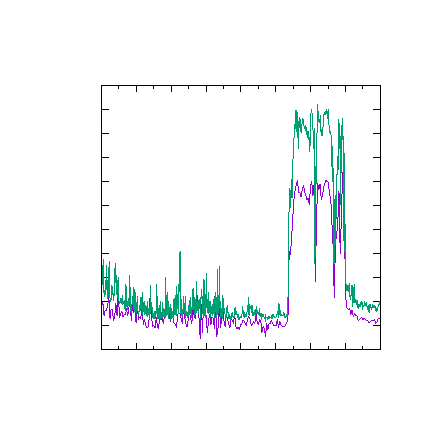
\includegraphics{../images/correlation_ts01}}%
    \gplfronttext
  \end{picture}%
\endgroup

  \hfill
  % GNUPLOT: LaTeX picture with Postscript
\begingroup
  \makeatletter
  \providecommand\color[2][]{%
    \GenericError{(gnuplot) \space\space\space\@spaces}{%
      Package color not loaded in conjunction with
      terminal option `colourtext'%
    }{See the gnuplot documentation for explanation.%
    }{Either use 'blacktext' in gnuplot or load the package
      color.sty in LaTeX.}%
    \renewcommand\color[2][]{}%
  }%
  \providecommand\includegraphics[2][]{%
    \GenericError{(gnuplot) \space\space\space\@spaces}{%
      Package graphicx or graphics not loaded%
    }{See the gnuplot documentation for explanation.%
    }{The gnuplot epslatex terminal needs graphicx.sty or graphics.sty.}%
    \renewcommand\includegraphics[2][]{}%
  }%
  \providecommand\rotatebox[2]{#2}%
  \@ifundefined{ifGPcolor}{%
    \newif\ifGPcolor
    \GPcolorfalse
  }{}%
  \@ifundefined{ifGPblacktext}{%
    \newif\ifGPblacktext
    \GPblacktexttrue
  }{}%
  % define a \g@addto@macro without @ in the name:
  \let\gplgaddtomacro\g@addto@macro
  % define empty templates for all commands taking text:
  \gdef\gplbacktext{}%
  \gdef\gplfronttext{}%
  \makeatother
  \ifGPblacktext
    % no textcolor at all
    \def\colorrgb#1{}%
    \def\colorgray#1{}%
  \else
    % gray or color?
    \ifGPcolor
      \def\colorrgb#1{\color[rgb]{#1}}%
      \def\colorgray#1{\color[gray]{#1}}%
      \expandafter\def\csname LTw\endcsname{\color{white}}%
      \expandafter\def\csname LTb\endcsname{\color{black}}%
      \expandafter\def\csname LTa\endcsname{\color{black}}%
      \expandafter\def\csname LT0\endcsname{\color[rgb]{1,0,0}}%
      \expandafter\def\csname LT1\endcsname{\color[rgb]{0,1,0}}%
      \expandafter\def\csname LT2\endcsname{\color[rgb]{0,0,1}}%
      \expandafter\def\csname LT3\endcsname{\color[rgb]{1,0,1}}%
      \expandafter\def\csname LT4\endcsname{\color[rgb]{0,1,1}}%
      \expandafter\def\csname LT5\endcsname{\color[rgb]{1,1,0}}%
      \expandafter\def\csname LT6\endcsname{\color[rgb]{0,0,0}}%
      \expandafter\def\csname LT7\endcsname{\color[rgb]{1,0.3,0}}%
      \expandafter\def\csname LT8\endcsname{\color[rgb]{0.5,0.5,0.5}}%
    \else
      % gray
      \def\colorrgb#1{\color{black}}%
      \def\colorgray#1{\color[gray]{#1}}%
      \expandafter\def\csname LTw\endcsname{\color{white}}%
      \expandafter\def\csname LTb\endcsname{\color{black}}%
      \expandafter\def\csname LTa\endcsname{\color{black}}%
      \expandafter\def\csname LT0\endcsname{\color{black}}%
      \expandafter\def\csname LT1\endcsname{\color{black}}%
      \expandafter\def\csname LT2\endcsname{\color{black}}%
      \expandafter\def\csname LT3\endcsname{\color{black}}%
      \expandafter\def\csname LT4\endcsname{\color{black}}%
      \expandafter\def\csname LT5\endcsname{\color{black}}%
      \expandafter\def\csname LT6\endcsname{\color{black}}%
      \expandafter\def\csname LT7\endcsname{\color{black}}%
      \expandafter\def\csname LT8\endcsname{\color{black}}%
    \fi
  \fi
    \setlength{\unitlength}{0.0500bp}%
    \ifx\gptboxheight\undefined%
      \newlength{\gptboxheight}%
      \newlength{\gptboxwidth}%
      \newsavebox{\gptboxtext}%
    \fi%
    \setlength{\fboxrule}{0.5pt}%
    \setlength{\fboxsep}{1pt}%
\begin{picture}(3888.00,3888.00)%
    \gplgaddtomacro\gplbacktext{%
      \csname LTb\endcsname%
      \put(814,686){\makebox(0,0)[r]{\strut{}$-10$}}%
      \put(814,1049){\makebox(0,0)[r]{\strut{}$0$}}%
      \put(814,1412){\makebox(0,0)[r]{\strut{}$10$}}%
      \put(814,1775){\makebox(0,0)[r]{\strut{}$20$}}%
      \put(814,2138){\makebox(0,0)[r]{\strut{}$30$}}%
      \put(814,2501){\makebox(0,0)[r]{\strut{}$40$}}%
      \put(814,2864){\makebox(0,0)[r]{\strut{}$50$}}%
      \put(814,3227){\makebox(0,0)[r]{\strut{}$60$}}%
      \put(946,554){\rotatebox{-45}{\makebox(0,0)[l]{\strut{}08:00}}}%
      \put(1264,554){\rotatebox{-45}{\makebox(0,0)[l]{\strut{}10:00}}}%
      \put(1582,554){\rotatebox{-45}{\makebox(0,0)[l]{\strut{}12:00}}}%
      \put(1900,554){\rotatebox{-45}{\makebox(0,0)[l]{\strut{}14:00}}}%
      \put(2219,554){\rotatebox{-45}{\makebox(0,0)[l]{\strut{}16:00}}}%
      \put(2537,554){\rotatebox{-45}{\makebox(0,0)[l]{\strut{}18:00}}}%
      \put(2855,554){\rotatebox{-45}{\makebox(0,0)[l]{\strut{}20:00}}}%
      \put(3173,554){\rotatebox{-45}{\makebox(0,0)[l]{\strut{}22:00}}}%
      \put(3491,554){\rotatebox{-45}{\makebox(0,0)[l]{\strut{}00:00}}}%
    }%
    \gplgaddtomacro\gplfronttext{%
      \csname LTb\endcsname%
      \put(176,1956){\rotatebox{-270}{\makebox(0,0){\strut{}Concentration [ppb]}}}%
      \put(2218,3557){\makebox(0,0){\strut{}January 25, 2016}}%
      \csname LTb\endcsname%
      \put(2504,3054){\makebox(0,0)[r]{\strut{}DOAS}}%
      \csname LTb\endcsname%
      \put(2504,2834){\makebox(0,0)[r]{\strut{}CLD}}%
    }%
    \gplbacktext
    \put(0,0){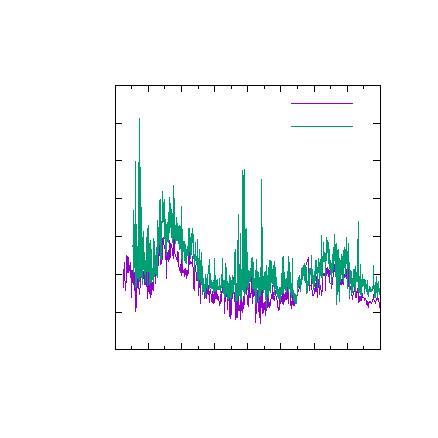
\includegraphics{../images/correlation_ts02}}%
    \gplfronttext
  \end{picture}%
\endgroup

  \caption{Time series of the \ch{NO} concentration during the two
    measurements on January 22 and January 25. Green depicts the
    chemiluminescence measurement, violet the DOAS measurement.}
  \label{fig:corr-ts}
\end{figure}
\begin{figure}[htbp]
  \centering
  % GNUPLOT: LaTeX picture with Postscript
\begingroup
  \makeatletter
  \providecommand\color[2][]{%
    \GenericError{(gnuplot) \space\space\space\@spaces}{%
      Package color not loaded in conjunction with
      terminal option `colourtext'%
    }{See the gnuplot documentation for explanation.%
    }{Either use 'blacktext' in gnuplot or load the package
      color.sty in LaTeX.}%
    \renewcommand\color[2][]{}%
  }%
  \providecommand\includegraphics[2][]{%
    \GenericError{(gnuplot) \space\space\space\@spaces}{%
      Package graphicx or graphics not loaded%
    }{See the gnuplot documentation for explanation.%
    }{The gnuplot epslatex terminal needs graphicx.sty or graphics.sty.}%
    \renewcommand\includegraphics[2][]{}%
  }%
  \providecommand\rotatebox[2]{#2}%
  \@ifundefined{ifGPcolor}{%
    \newif\ifGPcolor
    \GPcolorfalse
  }{}%
  \@ifundefined{ifGPblacktext}{%
    \newif\ifGPblacktext
    \GPblacktexttrue
  }{}%
  % define a \g@addto@macro without @ in the name:
  \let\gplgaddtomacro\g@addto@macro
  % define empty templates for all commands taking text:
  \gdef\gplbacktext{}%
  \gdef\gplfronttext{}%
  \makeatother
  \ifGPblacktext
    % no textcolor at all
    \def\colorrgb#1{}%
    \def\colorgray#1{}%
  \else
    % gray or color?
    \ifGPcolor
      \def\colorrgb#1{\color[rgb]{#1}}%
      \def\colorgray#1{\color[gray]{#1}}%
      \expandafter\def\csname LTw\endcsname{\color{white}}%
      \expandafter\def\csname LTb\endcsname{\color{black}}%
      \expandafter\def\csname LTa\endcsname{\color{black}}%
      \expandafter\def\csname LT0\endcsname{\color[rgb]{1,0,0}}%
      \expandafter\def\csname LT1\endcsname{\color[rgb]{0,1,0}}%
      \expandafter\def\csname LT2\endcsname{\color[rgb]{0,0,1}}%
      \expandafter\def\csname LT3\endcsname{\color[rgb]{1,0,1}}%
      \expandafter\def\csname LT4\endcsname{\color[rgb]{0,1,1}}%
      \expandafter\def\csname LT5\endcsname{\color[rgb]{1,1,0}}%
      \expandafter\def\csname LT6\endcsname{\color[rgb]{0,0,0}}%
      \expandafter\def\csname LT7\endcsname{\color[rgb]{1,0.3,0}}%
      \expandafter\def\csname LT8\endcsname{\color[rgb]{0.5,0.5,0.5}}%
    \else
      % gray
      \def\colorrgb#1{\color{black}}%
      \def\colorgray#1{\color[gray]{#1}}%
      \expandafter\def\csname LTw\endcsname{\color{white}}%
      \expandafter\def\csname LTb\endcsname{\color{black}}%
      \expandafter\def\csname LTa\endcsname{\color{black}}%
      \expandafter\def\csname LT0\endcsname{\color{black}}%
      \expandafter\def\csname LT1\endcsname{\color{black}}%
      \expandafter\def\csname LT2\endcsname{\color{black}}%
      \expandafter\def\csname LT3\endcsname{\color{black}}%
      \expandafter\def\csname LT4\endcsname{\color{black}}%
      \expandafter\def\csname LT5\endcsname{\color{black}}%
      \expandafter\def\csname LT6\endcsname{\color{black}}%
      \expandafter\def\csname LT7\endcsname{\color{black}}%
      \expandafter\def\csname LT8\endcsname{\color{black}}%
    \fi
  \fi
    \setlength{\unitlength}{0.0500bp}%
    \ifx\gptboxheight\undefined%
      \newlength{\gptboxheight}%
      \newlength{\gptboxwidth}%
      \newsavebox{\gptboxtext}%
    \fi%
    \setlength{\fboxrule}{0.5pt}%
    \setlength{\fboxsep}{1pt}%
\begin{picture}(7776.00,4320.00)%
    \gplgaddtomacro\gplbacktext{%
      \csname LTb\endcsname%
      \put(682,704){\makebox(0,0)[r]{\strut{}$-5$}}%
      \put(682,1039){\makebox(0,0)[r]{\strut{}$0$}}%
      \put(682,1374){\makebox(0,0)[r]{\strut{}$5$}}%
      \put(682,1709){\makebox(0,0)[r]{\strut{}$10$}}%
      \put(682,2044){\makebox(0,0)[r]{\strut{}$15$}}%
      \put(682,2380){\makebox(0,0)[r]{\strut{}$20$}}%
      \put(682,2715){\makebox(0,0)[r]{\strut{}$25$}}%
      \put(682,3050){\makebox(0,0)[r]{\strut{}$30$}}%
      \put(682,3385){\makebox(0,0)[r]{\strut{}$35$}}%
      \put(682,3720){\makebox(0,0)[r]{\strut{}$40$}}%
      \put(682,4055){\makebox(0,0)[r]{\strut{}$45$}}%
      \put(814,484){\makebox(0,0){\strut{}$-5$}}%
      \put(1752,484){\makebox(0,0){\strut{}$0$}}%
      \put(2690,484){\makebox(0,0){\strut{}$5$}}%
      \put(3628,484){\makebox(0,0){\strut{}$10$}}%
      \put(4565,484){\makebox(0,0){\strut{}$15$}}%
      \put(5503,484){\makebox(0,0){\strut{}$20$}}%
      \put(6441,484){\makebox(0,0){\strut{}$25$}}%
      \put(7379,484){\makebox(0,0){\strut{}$30$}}%
    }%
    \gplgaddtomacro\gplfronttext{%
      \csname LTb\endcsname%
      \put(176,2379){\rotatebox{-270}{\makebox(0,0){\strut{}Concentration (CLD) [ppb]}}}%
      \put(4096,154){\makebox(0,0){\strut{}Concentration (ICAD) [ppb]}}%
      \csname LTb\endcsname%
      \put(3322,3882){\makebox(0,0)[r]{\strut{}uncorrected}}%
      \csname LTb\endcsname%
      \put(3322,3662){\makebox(0,0)[r]{\strut{}fit uncorrected}}%
      \csname LTb\endcsname%
      \put(3322,3442){\makebox(0,0)[r]{\strut{}tail corrected}}%
      \csname LTb\endcsname%
      \put(3322,3222){\makebox(0,0)[r]{\strut{}fit tail corrected}}%
    }%
    \gplbacktext
    \put(0,0){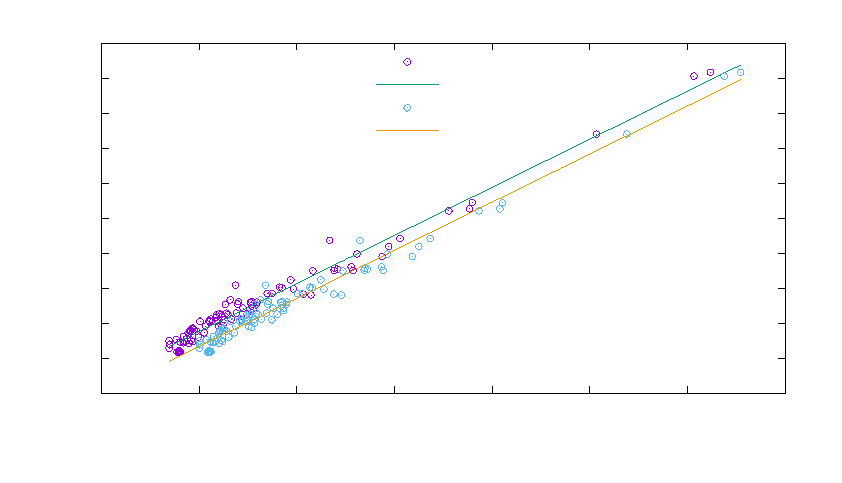
\includegraphics{../images/Correlation_corrected}}%
    \gplfronttext
  \end{picture}%
\endgroup

  \caption{Correlation plot between the DOAS instrument and a
    chemiluminescence monitor (CLD). Each data point depicts a
    \SI{30}{\minute} average.}
  \label{fig:cld-corr}
\end{figure}

All in all it seems that there are a few more stumbling blocks ahead
before this alternating measurement mode is ready for productive
use. The behavior of the converter after an ozone switch has to be
characterized thoroughly to explain and cope with all the observed
effects.

%%% Local Variables:
%%% mode: latex
%%% TeX-master: "../Bachelor"
%%% End:
